%%%%%%%%%%%%%%%%%%%%%%%%%%%%%%%%%%%%%%%%%%%%%%%%%%%%%%%%%%%%%%%%%%%%%%%%%%%%%%%
% Chapter 3: Data Pipeline
%%%%%%%%%%%%%%%%%%%%%%%%%%%%%%%%%%%%%%%%%%%%%%%%%%%%%%%%%%%%%%%%%%%%%%%%%%%%%%%

\chapter{Data Pipeline}
\label{ch:data_pipeline}

This chapter details the node-feature-based data processing pipeline that converts raw surveillance videos into dynamic graph sequences suitable for the Temporal DGNN model. The pipeline is implemented in Python and leverages YOLOv8 for vehicle detection and PyTorch Geometric for graph representation.

\section{Pipeline Overview}

The data pipeline consists of five main stages:

\begin{enumerate}
    \item \textbf{Video Discovery:} Scan input directory for video files organized by split and class
    \item \textbf{Vehicle Detection:} Apply YOLOv8 to detect vehicles in each frame
    \item \textbf{Vehicle Tracking:} Assign consistent IDs to vehicles across frames
    \item \textbf{Graph Construction:} Build per-frame PyG graphs with dynamic node counts
    \item \textbf{Data Storage:} Save graphs as \texttt{.pt} files (30 per video) with CSV manifests
\end{enumerate}

Figure~\ref{fig:pipeline_flow} illustrates the complete pipeline flow.

\begin{figure}[H]
    \centering
    % Pipeline Flow Diagram
\begin{tikzpicture}[
    node distance=0.6cm and 1cm,
    box/.style={
        rectangle,
        rounded corners=3pt,
        minimum width=2cm,
        minimum height=0.8cm,
        align=center,
        draw=black,
        thick,
        font=\footnotesize
    },
    smallbox/.style={
        rectangle,
        rounded corners=2pt,
        minimum width=1.5cm,
        minimum height=0.5cm,
        align=center,
        draw=black,
        font=\tiny
    },
    input/.style={box, fill=cyan!25},
    process/.style={box, fill=green!25},
    output/.style={box, fill=orange!25},
    data/.style={smallbox, fill=purple!20},
    arrow/.style={-Stealth, thick}
]

% Stage 1: Input
\node[input] (video) at (0, 2.5) {Video Files};
\node[data, below=0.2cm of video] (d1) {30 frames};

% Stage 2: Frame Extraction
\node[process] (frames) at (2.5, 2.5) {Frame Extract};
\node[data, below=0.2cm of frames] (d2) {RGB};

% Stage 3: YOLO Detection
\node[process] (yolo) at (5, 2.5) {YOLOv8};
\node[data, below=0.2cm of yolo] (d3) {Boxes};

% Stage 4: Vehicle Tracking
\node[process] (track) at (7.5, 2.5) {Tracking};
\node[data, below=0.2cm of track] (d4) {IDs};

% Stage 5: Graph Construction
\node[process] (graph) at (5, 0) {Graph Build};

% Sub-processes
\node[smallbox, fill=yellow!20] (nodes) at (2.5, 0) {Features};
\node[smallbox, fill=yellow!20] (edges) at (7.5, 0) {Edges};

% Stage 6: Output
\node[output] (pt) at (10, 0) {.pt Files};
\node[output] (csv) at (10, 2.5) {Manifest};

% Arrows - main flow
\draw[arrow] (video) -- (frames);
\draw[arrow] (frames) -- (yolo);
\draw[arrow] (yolo) -- (track);
\draw[arrow] (track) -- (csv);
\draw[arrow] (track) |- (graph);

% Arrows - graph construction
\draw[arrow] (nodes) -- (graph);
\draw[arrow] (edges) -- (graph);
\draw[arrow] (graph) -- (pt);

\end{tikzpicture}

    \caption{Data pipeline flowchart showing the transformation from raw video to PyTorch Geometric graph sequence.}
    \label{fig:pipeline_flow}
\end{figure}

\section{Video Processing}

Videos are organized by split (Training/Validation/Testing) and class (Normal/Accident). Each video is processed to extract exactly 30 frames using YOLOv8 with confidence threshold 0.3 for vehicle classes 2, 3, 5, 7 (car, motorcycle, bus, truck).

\section{Vehicle Detection}

\subsection{YOLO Configuration}

We use YOLOv8 (nano variant) for efficient vehicle detection:

\begin{table}[H]
\centering
\caption{YOLO Detection Configuration}
\label{tab:yolo_config}
\begin{tabular}{ll}
\toprule
\textbf{Parameter} & \textbf{Value} \\
\midrule
Model & YOLOv8n (nano) \\
Confidence Threshold & 0.3 \\
Vehicle Classes & 2 (car), 3 (motorcycle), 5 (bus), 7 (truck) \\
Device & CUDA GPU \\
\bottomrule
\end{tabular}
\end{table}

YOLO outputs bounding boxes, centroids, class IDs, and confidence scores for each detected vehicle.


\section{Vehicle Tracking}

Centroid-based tracking maintains consistent vehicle IDs across frames using distance matching (max\_distance=100 pixels, max\_disappeared=10 frames). The Hungarian algorithm matches detections to existing tracks.


\section{Graph Construction}

\subsection{Dynamic Graph Representation}

Unlike fixed-size matrix approaches, each frame produces a graph containing \textbf{only the vehicles present in that frame}. This eliminates padding and missing value handling:

\begin{itemize}
    \item \textbf{Node Features:} $\mat{X}_t \in \R^{N_t \times 8}$ where $N_t$ is the number of vehicles in frame $t$
    \item \textbf{Edge Index:} Sparse representation of fully-connected graph
    \item \textbf{Edge Weight:} Euclidean distance between centroids
    \item \textbf{Node IDs:} Tracking IDs for temporal consistency
\end{itemize}

\subsection{Node Features (8 dimensions)}

Each node (vehicle) has 8 features:

\begin{table}[H]
\centering
\caption{Node Feature Specification}
\label{tab:node_features}
\begin{tabular}{clll}
\toprule
\textbf{Index} & \textbf{Feature} & \textbf{Description} & \textbf{Range} \\
\midrule
0 & centroid\_x & X-coordinate of bounding box center & $[0, \text{width}]$ \\
1 & centroid\_y & Y-coordinate of bounding box center & $[0, \text{height}]$ \\
2 & bbox\_x & Top-left X coordinate & $[0, \text{width}]$ \\
3 & bbox\_y & Top-left Y coordinate & $[0, \text{height}]$ \\
4 & bbox\_w & Bounding box width & $[0, \text{width}]$ \\
5 & bbox\_h & Bounding box height & $[0, \text{height}]$ \\
6 & class\_id & YOLO class ID & $\{2, 3, 5, 7\}$ \\
7 & timestamp & Normalized time: frame\_index / 29 & $[0, 1]$ \\
\bottomrule
\end{tabular}
\end{table}



\subsection{Edge Construction}

Edges connect all pairs of vehicles in each frame with weights based on Euclidean distance:

\begin{equation}
    \text{edge\_weight}_{ij} = \|\vect{c}_i - \vect{c}_j\|_2 = \sqrt{(c_{x,i} - c_{x,j})^2 + (c_{y,i} - c_{y,j})^2}
\end{equation}

For a frame with $N_t$ nodes, the fully connected graph has $N_t \times (N_t - 1)$ directed edges.

Figure~\ref{fig:graph_construction} illustrates the graph construction process.

\begin{figure}[H]
    \centering
    % Graph Construction Diagram
\begin{tikzpicture}[
    node distance=1cm,
    vertex/.style={
        circle,
        draw=black,
        thick,
        minimum size=0.8cm,
        font=\small,
        align=center
    },
    present/.style={vertex, fill=green!40},
    arrow/.style={-Stealth, thick}
]

% Title
\node[font=\bfseries] at (6, 5) {Graph Construction from Detections};

% Left side: Detections
\node[font=\small\bfseries] at (1.5, 4) {Frame Detections};

% Detected vehicles (only present ones)
\node[present] (v0) at (0, 2.5) {V0};
\node[present] (v1) at (3, 2.5) {V1};
\node[present] (v2) at (1.5, 0.8) {V2};

% Edges with distances
\draw[thick, blue] (v0) -- node[above, font=\scriptsize] {198} (v1);
\draw[thick, blue] (v0) -- node[left, font=\scriptsize] {155} (v2);
\draw[thick, blue] (v1) -- node[right, font=\scriptsize] {352} (v2);

% Arrow
\draw[arrow, very thick] (4, 1.8) -- (5, 1.8);

% Right side: PyG Data
\node[font=\small\bfseries] at (9, 4) {PyG Data Object};

% Data box
\draw[thick, rounded corners] (5.5, 0.5) rectangle (12.5, 3.5);

% x: node features
\node[font=\scriptsize, anchor=west] at (5.7, 3.1) {\textbf{x} $[3, 8]$:};
\node[font=\tiny, anchor=west] at (7.2, 3.1) {[[37, 230, 0, 215, 74, 31, 2, 0.0],};
\node[font=\tiny, anchor=west] at (7.5, 2.8) {[175, 249, 130, 221, 91, 57, 2, 0.0],};
\node[font=\tiny, anchor=west] at (7.5, 2.5) {[828, 410, 790, 368, 76, 84, 3, 0.0]]};

% edge_index
\node[font=\scriptsize, anchor=west] at (5.7, 2.1) {\textbf{edge\_index} $[2, 6]$:};
\node[font=\tiny, anchor=west] at (8.2, 2.1) {[[0,0,1,1,2,2], [1,2,0,2,0,1]]};

% edge_weight
\node[font=\scriptsize, anchor=west] at (5.7, 1.7) {\textbf{edge\_weight} $[6]$:};
\node[font=\tiny, anchor=west] at (8.2, 1.7) {[198, 155, 198, 352, 155, 352]};

% node_ids
\node[font=\scriptsize, anchor=west] at (5.7, 1.3) {\textbf{node\_ids} $[3]$:};
\node[font=\tiny, anchor=west] at (8.2, 1.3) {[0, 1, 2]};

% t
\node[font=\scriptsize, anchor=west] at (5.7, 0.9) {\textbf{t}:};
\node[font=\tiny, anchor=west] at (6.5, 0.9) {0 (frame index)};

% Legend
\node[present, minimum size=0.4cm] at (5, -0.2) {};
\node[font=\scriptsize, right] at (5.3, -0.2) {Present vehicle (node)};
\node[font=\scriptsize, blue] at (10, -0.2) {Edge = Euclidean distance};

\end{tikzpicture}

    \caption{Graph construction from vehicle detections. Nodes represent present vehicles only, edges represent spatial distances.}
    \label{fig:graph_construction}
\end{figure}


\section{PyTorch Geometric Data Format}

Each frame graph is stored as a PyTorch Geometric \texttt{Data} object with fields: \texttt{x} (node features [N, 8]), \texttt{edge\_index} ([2, E]), \texttt{edge\_weight} ([E]), \texttt{node\_ids} ([N]), and \texttt{t} (frame index).

Each video produces 30 \texttt{.pt} files organized by split and class. CSV manifests track video metadata (path, label, vehicle counts).

Figure~\ref{fig:hdf5_structure} illustrates the file structure.

\begin{figure}[H]
    \centering
    % PyG File Structure Diagram
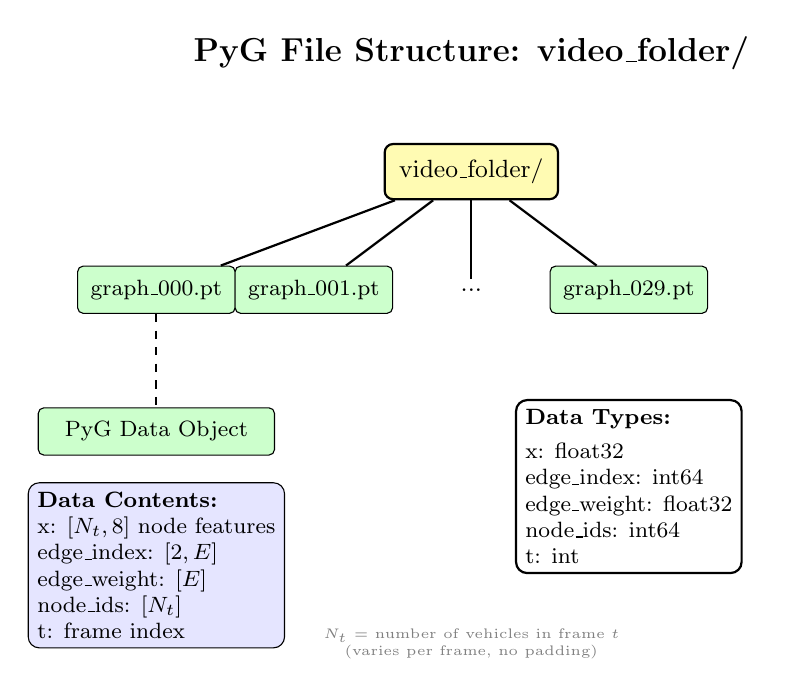
\begin{tikzpicture}[
    folder/.style={
        rectangle,
        rounded corners=3pt,
        draw=black,
        thick,
        fill=yellow!30,
        font=\small,
        minimum height=0.7cm,
        minimum width=2.2cm,
        align=center
    },
    file/.style={
        rectangle,
        rounded corners=2pt,
        draw=black,
        fill=green!20,
        font=\footnotesize,
        minimum height=0.6cm,
        minimum width=2cm,
        align=center
    },
    arrow/.style={draw, thick, -}
]

% Title
\node[font=\bfseries\large] at (4, 3) {PyG File Structure: video\_folder/};

% Root
\node[folder] (root) at (4, 1.5) {video\_folder/};

% Graph files
\node[file] (g0) at (0, 0) {graph\_000.pt};
\node[file] (g1) at (2, 0) {graph\_001.pt};
\node[font=\small] (dots) at (4, 0) {...};
\node[file] (g29) at (6, 0) {graph\_029.pt};

% Connect root to files
\draw[arrow] (root) -- (g0);
\draw[arrow] (root) -- (g1);
\draw[arrow] (root) -- (dots);
\draw[arrow] (root) -- (g29);

% Expand one graph file
\node[file, minimum width=3cm] (data) at (0, -1.8) {PyG Data Object};

\draw[arrow, dashed] (g0) -- (data);

% Data object contents
\node[font=\footnotesize, align=left, fill=blue!10, draw, rounded corners] at (0, -3.5) {
    \textbf{Data Contents:}\\
    x: $[N_t, 8]$ node features\\
    edge\_index: $[2, E]$\\
    edge\_weight: $[E]$\\
    node\_ids: $[N_t]$\\
    t: frame index
};

% Data type annotations box
\node[font=\footnotesize, align=left, fill=white, draw, rounded corners, thick] at (6, -2.5) {
    \textbf{Data Types:}\\[0.1cm]
    x: float32\\
    edge\_index: int64\\
    edge\_weight: float32\\
    node\_ids: int64\\
    t: int
};

% Note about dynamic size
\node[font=\tiny, gray, align=center] at (4, -4.5) {$N_t$ = number of vehicles in frame $t$\\(varies per frame, no padding)};

\end{tikzpicture}

    \caption{PyTorch Geometric file structure. Each frame produces a separate \texttt{.pt} file containing the graph data object.}
    \label{fig:hdf5_structure}
\end{figure}

Graph sequences are loaded by iterating through 30 \texttt{.pt} files per video. The \texttt{node\_ids} field enables temporal alignment by sorting nodes by tracking IDs before processing.

\section{Data Augmentation}

Data augmentation is applied \textbf{only to anomalous training samples} to address class imbalance.

\subsection{Augmentation Strategies}

\begin{enumerate}
    \item \textbf{Original:} Unmodified video (no suffix)
    \item \textbf{Brightness:} Adjusted lighting conditions (suffix: \texttt{\_bright})
    \item \textbf{Horizontal Flip:} Mirror transformation (suffix: \texttt{\_flip})
    \item \textbf{Spatial Shift:} Left-shifted frames (suffix: \texttt{\_shift\_left})
\end{enumerate}

\subsection{Augmentation Statistics}

\begin{table}[H]
\centering
\caption{Training Set Augmentation Breakdown}
\label{tab:augmentation_stats}
\begin{tabular}{lccc}
\toprule
\textbf{Class} & \textbf{Original} & \textbf{Augmented} & \textbf{Total} \\
\midrule
Normal & 638 & 0 & 638 \\
Anomalous & 51 & 153 (3 variants each) & 204 \\
\midrule
\textbf{Total} & \textbf{689} & \textbf{153} & \textbf{842} \\
\bottomrule
\end{tabular}
\end{table}

Figure~\ref{fig:data_augmentation} visualizes the augmentation strategies.

\begin{figure}[H]
    \centering
    % Data Augmentation Diagram
\begin{tikzpicture}[
    frame/.style={
        rectangle,
        draw=black,
        rounded corners,
        minimum width=1.8cm,
        minimum height=1.4cm,
        font=\tiny
    },
    arrow/.style={-Stealth, thick}
]

% Title
\node[font=\bfseries] at (5, 5) {Data Augmentation (4$\times$)};

% Original frame
\node[frame, fill=gray!20] (orig) at (0, 2.5) {};
\node[font=\footnotesize\bfseries, above=0.1cm of orig] {Original};
\draw[fill=blue!30, draw=black] (-0.3, 2.2) rectangle (0.2, 2.6);
\draw[fill=blue!30, draw=black] (0, 2.0) rectangle (0.3, 2.2);

% Brightness adjusted
\node[frame, fill=yellow!30] (bright) at (4, 4) {};
\node[font=\footnotesize, above=0.1cm of bright] {Bright};
\draw[fill=blue!50, draw=black] (3.7, 3.7) rectangle (4.2, 4.1);
\draw[fill=blue!50, draw=black] (4, 3.5) rectangle (4.3, 3.7);

% Horizontal flip
\node[frame, fill=green!20] (flip) at (4, 1) {};
\node[font=\footnotesize, above=0.1cm of flip] {Flip};
\draw[fill=blue!30, draw=black] (3.8, 0.7) rectangle (4.3, 1.1);
\draw[fill=blue!30, draw=black] (3.7, 0.5) rectangle (4, 0.7);

% Spatial shift
\node[frame, fill=orange!20] (shift) at (8, 2.5) {};
\node[font=\footnotesize, above=0.1cm of shift] {Shift};
\draw[fill=blue!30, draw=black] (7.2, 2.2) rectangle (7.7, 2.6);
\draw[fill=blue!30, draw=black] (7.5, 2.0) rectangle (7.8, 2.2);

% Arrows
\draw[arrow] (orig) -- (bright);
\draw[arrow] (orig) -- (flip);
\draw[arrow] (orig) -- (shift);

% Statistics box
\node[draw, rounded corners, fill=white, font=\footnotesize, align=left] at (11, 2.5) {
    \textbf{Augmentation:}\\
    51 Anomalous $\times$ 4\\
    = 204 training samples
};

\end{tikzpicture}

    \caption{Data augmentation strategies applied to anomalous training videos. Each original video generates 4 variants (including original) for class balancing.}
    \label{fig:data_augmentation}
\end{figure}


\section{Pipeline Summary}

\begin{table}[H]
\centering
\caption{Pipeline Processing Summary}
\label{tab:pipeline_summary}
\begin{tabular}{ll}
\toprule
\textbf{Metric} & \textbf{Value} \\
\midrule
Total videos processed & 1,176 \\
Training videos & 842 (638 Normal + 204 Anomalous) \\
Validation videos & 128 \\
Test videos & 206 \\
Frames per video & 30 (fixed) \\
Node features per vehicle & 8 \\
Vehicle classes detected & 4 (car, motorcycle, bus, truck) \\
YOLO confidence threshold & 0.3 \\
Storage format & PyTorch Geometric \texttt{.pt} files \\
Graph type & Fully connected (per frame) \\
\bottomrule
\end{tabular}
\end{table}
